% !TeX spellcheck = sk_SK-Slovak
\documentclass[a4paper]{article}
\usepackage[slovak]{babel}
\usepackage[utf8]{inputenc}
\usepackage[T1]{fontenc}
\usepackage{a4wide}
\usepackage{amsmath}
\usepackage{amsfonts}
\usepackage{amssymb}
\usepackage{mathrsfs}
\usepackage[small,bf]{caption}
\usepackage{subcaption}
\usepackage{xcolor}
\usepackage{graphicx}
\usepackage{enumerate}
\usepackage{hyperref}



\pagestyle{empty}
\setlength{\parindent}{0pt}

\newenvironment{modenumerate}
{\enumerate\setupmodenumerate}
{\endenumerate}

\newif\ifmoditem
\newcommand{\setupmodenumerate}{%
	\global\moditemfalse
	\let\origmakelabel\makelabel
	\def\moditem##1{\global\moditemtrue\def\mesymbol{##1}\item}%
	\def\makelabel##1{%
		\origmakelabel{##1\ifmoditem\rlap{\mesymbol}\fi\enspace}%
		\global\moditemfalse}%
}

\makeatletter
\def\@seccntformat#1{%
	\expandafter\ifx\csname c@#1\endcsname\c@section\else
	\csname the#1\endcsname\quad
	\fi}
\makeatother

\begin{document} 
	
\pagenumbering{arabic}
\pagestyle{plain}

\begin{center}
	\sc\large
	Umelá inteligencia - cvičenia 10
\end{center}

Autor: Marián Kravec

\section{Úloha 2}

\subsection*{Môj model}

Budeme modelovať čudný semafor, pričom to čo pozorujeme, je či autá prechádzajú cez križovatku.
\\

Náš model bude mať 3 skryté stavy: červená (č), oranžová (o) a zelená (z).

Našou pozorovaná premenná bude mať iba 2 hodnoty: autá idú (ai), autá stoja (as).
\\

Grafická vizualizácia modelu:

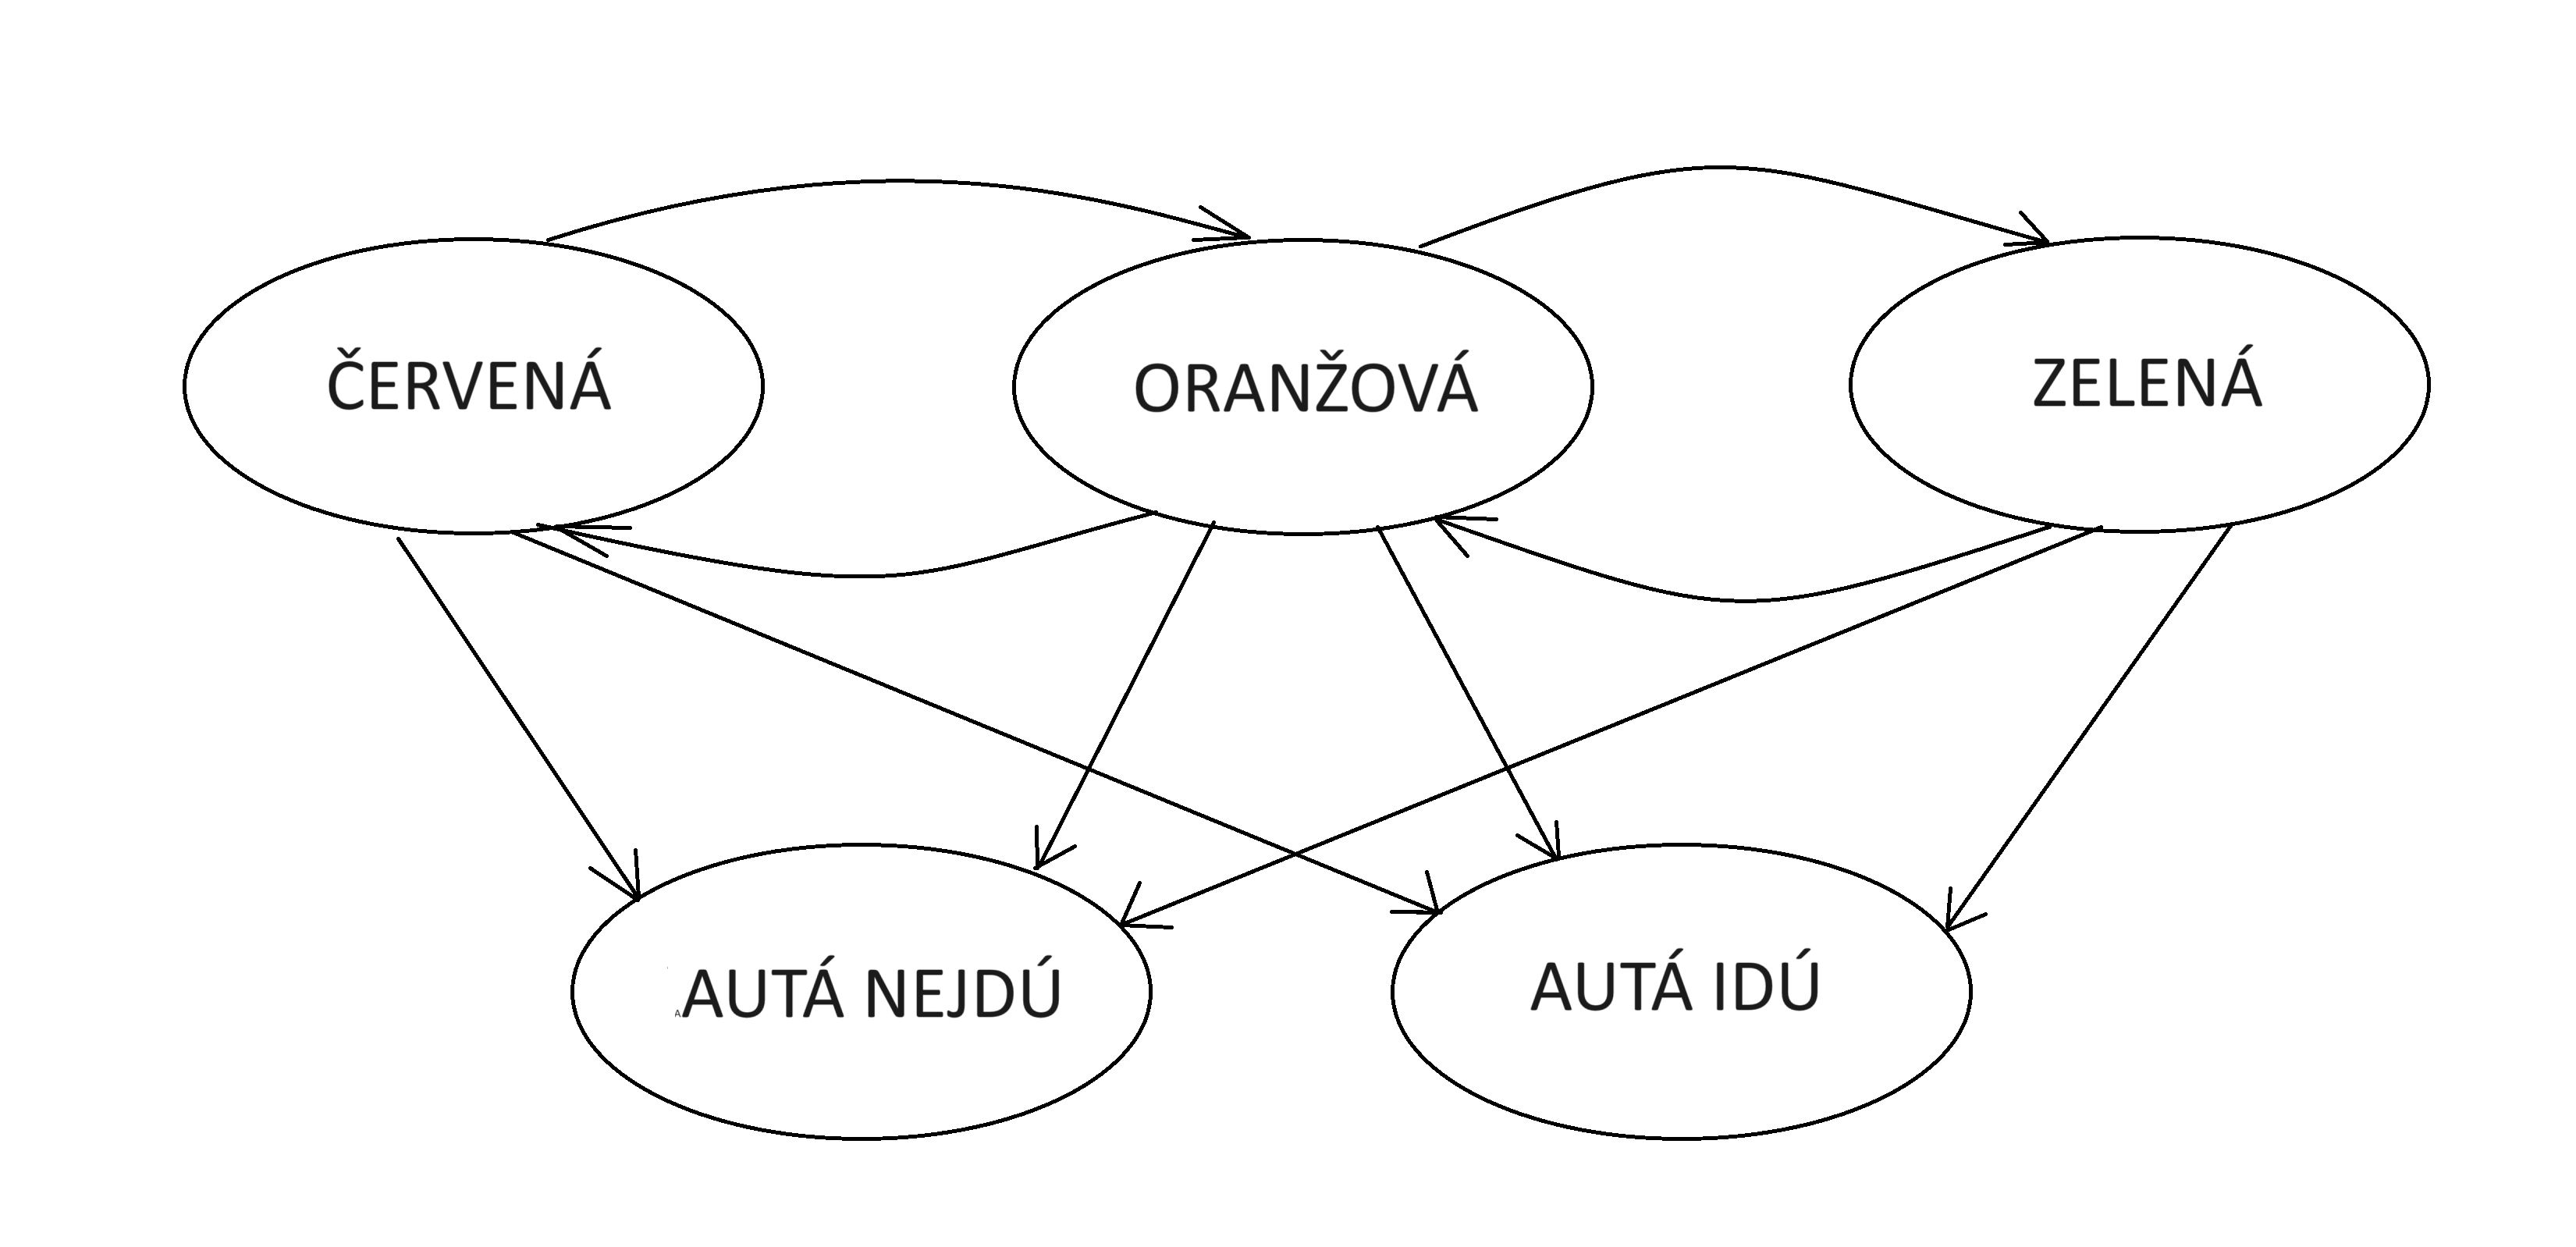
\includegraphics[width=\textwidth]{HMM.png}

Inicialne začne vždy kvôli bezpečnosti cestnej premávky v stave červená.
\\ 

Tranzičná matica bude nasledovná:

\begin{table}[h!]
	\begin{tabular}{|l|l|l|l|}
		\hline
		$s_i$ \char`\\ $s_{i+1}$ & č   & o   & z   \\ \hline
		č                    & 0.7 & 0.3 & 0   \\ \hline
		o                    & 0.3 & 0.4 & 0.3 \\ \hline
		z                    & 0   & 0.2 & 0.8 \\ \hline
	\end{tabular}
\end{table}

Čiže s červenej nikdy neprejde hneď na zelenú (a naopak). Ale z oranžovej sa môže vrátiť aj späť do stavu z ktoré ho sa do oranžovej dostal (zvláštnosť tohto semaforu).
\\

Emisná matica je nasledovná:

\begin{table}[h!]
	\begin{tabular}{|l|l|l|}
		\hline
		$s_i$ \char`\\ $v_i$ & as   & ai     \\ \hline
		č                    & 0.95 & 0.05  \\ \hline
		o                    & 0.3  & 0.7  \\ \hline
		z                    & 0.01 & 0.99  \\ \hline
	\end{tabular}
\end{table}

Na červenú ide len pár odvážlivcov, na oranžovú už viac ako polovica a na zelenú takmer všetci.
\\

Po vygenerovaní 10000 krokov modelu, sme získali pozorovania ktoré majú skóre: $-5189.26$

\newpage

\subsection*{Parťákov model}

Parťák: Viktória Ondrejová
\\

Popis modelu a jeho matice:
\\

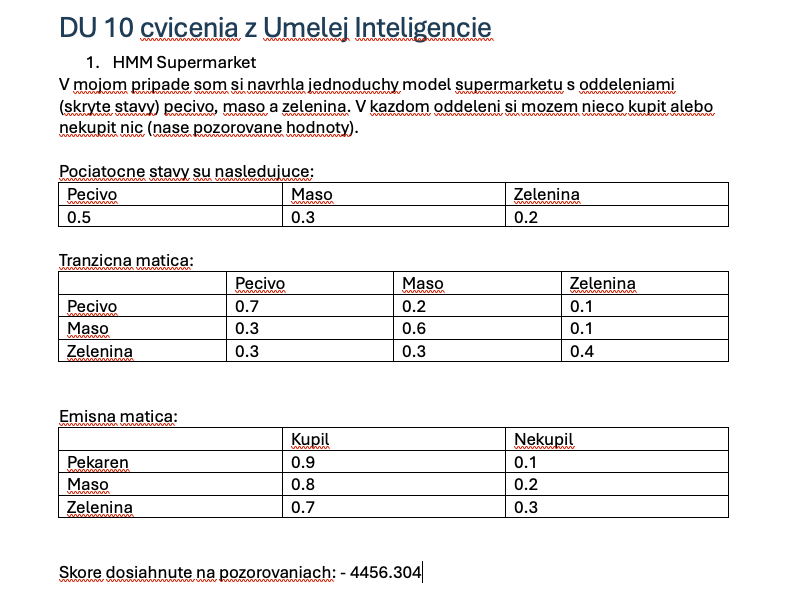
\includegraphics[width=\textwidth]{model_viky.png}

\newpage

\subsection*{Trenovanie parťákovho modelu}

Po pokuse o trénovanie tohto modelu sme dostali následné matice:

Odhadnutá tranzičná matica:

\begin{table}[h!]
	\begin{tabular}{|l|l|l|l|}
		\hline
		$s_i$ \char`\\ $s_{i+1}$ & Pečivo   & Mäso   & Zelenina   \\ \hline
		Pečivo              & 0.001 & 0.748 & 0.25   \\ \hline
		Mäso                & 0 & 0.74 & 0.26 \\ \hline
		Zelenina            & 0.203   & 0.796 & 0.001 \\ \hline
	\end{tabular}
\end{table}

Odhadnutá emisná matica:

\begin{table}[h!]
	\begin{tabular}{|l|l|l|}
		\hline
		$s_i$ \char`\\ $v_i$ & Kúpil  & Nekúpil     \\ \hline
		Pečivo                & 0.661 & 0.339  \\ \hline
		Mäso               & 0.906  & 0.094  \\ \hline
		Zelenina               & 0.57 & 0.43  \\ \hline
	\end{tabular}
\end{table}

Výsledné skóre: -4599.50
\\

Porovnanie skutočných a odhadnutých stavov

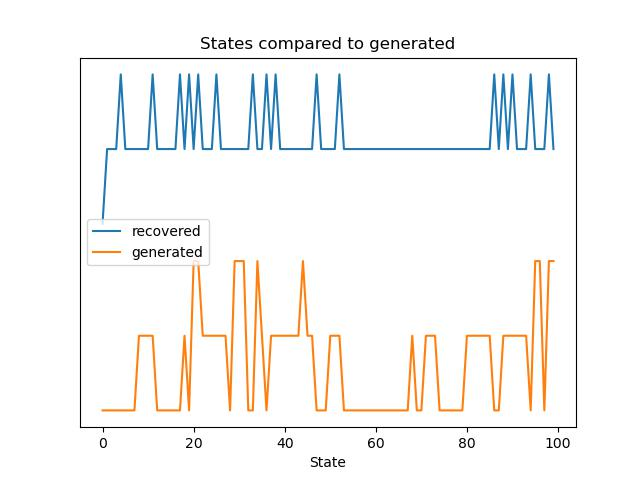
\includegraphics[width=0.8\textwidth]{odhad_stavov.jpg}

Vidíme, že tranzičná matica je odhadnutá pomerne zle, kedy model nikdy nechce ostať v stave Pečivo alebo Zelenina a zo stavu Mäso sa nikdy nedostane priamo do stavu Pečivo. Toto správanie môžeme pozorovať aj na grafe porovnávajúcom stavy. Toto správanie je s najväčšou pravdepodobnosťou spôsobené kombináciou nešťastnej náhody a faktu, že tento model je vo všeobecnosti ťažko odhadnuteľný keďže bez ohľadu na stav v ktorom sa nachádzame, je nadpolovičná pravdepodobnosť kúpi produktu pričom tieto pravdepodobnosti nie sú pre jednotlivé stavy veľmi odlišné, zo tohto vyplýva, že je pomerne náročné určiť bod kedy sa stav mení ak sa stavy správajú podobne, toto správanie je ešte amplifikované častými zmenami stavu originálneho modelu ktoré ešte viac mažú už aj tak malý rozdiel medzi správaním modelu v danom stave.
\\

Prekvapivo emisná matica je pomerne rozumná čo sa však dalo čakať keďže jednoducho stačilo aby platilo, že pravdepodobnosť kúpi je pre každý stav nadpolovičná.

\end{document}